\section{FaceLift Framework}
\label{sec:framework}

\begin{table}[t]
	\resizebox{0.7\linewidth}{!}{
		\begin{tabular}{l|p{8cm}}
			\textbf{Symbol} & \textbf{Meaning}\\
			$I_i$    & Original urban scene \\
			$Y$    & Set of annotation classes for urban scenes (e.g., beautiful, ugly)\\
			$y_i$    & Annotation class in $Y$ (e.g., beautiful) \\
			$\hat{I_j}$ & Template scene (synthetic image) \\
			$I'$ & Target Image \\
			$C$ & Beauty Classifier \\
			%$R$ & Images acquired by rotating Street view camera \\
			%$T$ & Images acquired by translating street view camera\\
			%$\rho$ & Similarity bound below which smart augmentation chooses translated images \\
			& \\
%			\textbf{term} & \textbf{stands for}\\
%			\textit{Template Image} $\hat{I_j}$    & A synthetic transformation of input image $I$ towards the class $y_j$ \\
%			\textit{Target Image} $I'$    & The natural image which is most visually similar to the template image \\
%		%	\textit{ Data Clustering}    & A process which groups images in $X$ according to visual similarity (e.g urban vs rural)\\
%			\textit{Data Augmentation}    & A process of data expansion which looks for images taken in the surroundings of the georeferenced images in $X$\\
%			\textit{Classifier}   & A deep-learning framework that is able to classify images into one of the classes in $Y$\\
%			\textit{Generator} $(GAN)$    & A deep-learning based image generator \\% framework to produce images similar to the ones in  $X$\\
%			$DGN-AM$    & A framework that, given the GAN and the Classifier, transforms an input image into the template image.\\
	\end{tabular}}
	\caption{Notations}\label{notations}
\end{table}

 \begin{figure*}[ht]
	\centering
	\includegraphics[width=\linewidth]{Plot/facelift-pipeline-2x.png}
	\caption{An illustration of the FaceLift framework.}
	\label{fig:framework}
\end{figure*}

%****************************************
The main goal of FaceLift is to beautify an existing urban scene. To meet that goal, it performs five steps: 
\begin{description}
	\item \textbf{Step 1 Curating urban scenes.} Deep learning systems need considerable amounts of training data. To augment our initial set of data, we develop a new way of curating and augmenting the number of annotated images.  
	\item \textbf{Step 2 Training a beauty classifier.} We design and train a deep learning model that is able to distinguish beautiful urban scenes from non-beautiful ones. 
	\item \textbf{Step 3 Generating a synthetic beautified scene.} Based on our classifier's learned representation of beauty, we train a generative model that is able to generate a  beautified version 
of an urban scene in input. 
	\item \textbf{Step 4 Retrieving a realistic beautified scene.} The generated image has a ``synthetic look'' and, as such, does not look realistic (Figure\ref{fig:framework}). To fix that, we retrieve the image in our set  most similar to the generated image. 
	\item \textbf{Step 5 Identifying the urban elements characterizing the beautified scene.} In the final step, the framework explains changes introduced in the transformation process in terms of addition and removal of specific urban elements. 
\end{description}
%1) curating urban scenes; 2) training a beauty classifier; 3) generating a synthetic beautified scene; 4) returning a realistic beautified scene; and 5) identifying the urban elements characterizing the beautified scene. 
%\ns{You need a bit more detail here. First sentence says what you are going to achieve. But you need to motivate why these specific five steps will achieve this goal.}


%****************************************
\subsection*{Step 1 Curating Urban Scenes}
\label{Sec:dataset}
To begin with, we need highly curated training data with labels reflecting urban beauty. We start with the  Place Pulse dataset that contains 100k Google Street Views across 56 cities around the world~\cite{dubey2016deep}. These scenes are labeled in terms of whether the corresponding places are likely to be perceived beautiful, depressing, rich, and safe. We focus only on those scenes that are labeled in terms of beauty and that have at least three judgments. This leave us with roughly  20,000 scenes. To transform judgments into beauty scores, we use the TrueSkill algorithm~\cite{herbrich2007trueskill}, which gives us a way of partitioning the scenes into two sets (Figure \ref{fig:Trueskill}): one containing beautiful scenes, and the other containing ugly scenes. The resulting set of scenes is too small for training any deep learning model without avoiding over-fitting though. As such, we need to augment such a set. 

We do so in two ways. First, we feed each scene's location into the Google Streetview API to obtain  the snapshots of the same location at different camera angles (i.e., at $\theta \in {-30^{\circ}, -15^{\circ} , 15^{\circ} , 30^{\circ} }$). However, the resulting dataset is still too small for robust training. Therefore, again, we feed each scene's location into the Google Streetview API, but we now do so to obtain other scenes at  distance $d \in \{10,20,40,60\}$ meters.  This will greatly expand our set of scenes, but it might do so at the price of introducing scenes whose beauty scores have little to do with the original scene's. To fix that, we take only the scenes that are \emph{similar} to the original one (we call this way of augmenting ``conservative translation''). To compute the similarity between a pair of scenes, we represent the two scenes with visual features derived from the FC7 layer of PlacesNet and compute the similarity between the two corresponding feature vectors~\cite{zhou2014learning}. For all scenes at increasing distance $d \in \{10,20,40,60\}$ meters,  we take only those whose similarity scores with the original scene is above a threshold. In a conservative fashion, we choose that threshold to be the median similarity between rotated and original scenes (those of the first augmentation step). 

To make sure this additional augmentation has not introduced any unwanted noise, we consider  two sets of scenes: one containing those that have been taken during this last step, i.e., the one with high similarity to the original scenes (\emph{taken-set}), and the other containing those that have been filtered away (\emph{filtered-set}). Each scene is then scored with PlacesNet~\cite{zhou2014learning} and is represented with the five most confident scene labels. We then aggregate labels at set level by computing each label's frequency on the \emph{taken-set} %minus that on the 
and on the \emph{filtered-set}. Finally, we characterize each label's propensity to be correctly augmented as: 
$ \textrm{prone}(label)= fr(label,\textrm{\emph{taken-set}}) - fr(label,\textrm{\emph{filtered-set}}).$
This reflects the extent to which a scene with a given label is prone to be augmented or not. From Figure~\ref{fig:augmentationSimilarity}, we find that, as one would expect, scenes that contain highways, fields and bridges can be augmented at increasing distances while still showing resemblances to the original scene; by contrast, scenes that contain gardens, residential neighborhoods, plazas, and skyscrapers cannot be easily augmented, as they are often found in high density parts of the city in which diversity within short distances might well be experienced. 

%\ns{You probably want to reword this: It is amenable to augmentation, not prone to. Also why is this being done at a set level? If you always find bridges next to viaducts and viaducts next to bridges, and if your translation step moves from one to another, then the set-level score will not detect this. If instead you check whether the placesnet\_label of the translated image is the same as that of the original, then you are OK, as long as placesnet\_label can be be believed.}

\begin{figure}[t!]
	\centering
	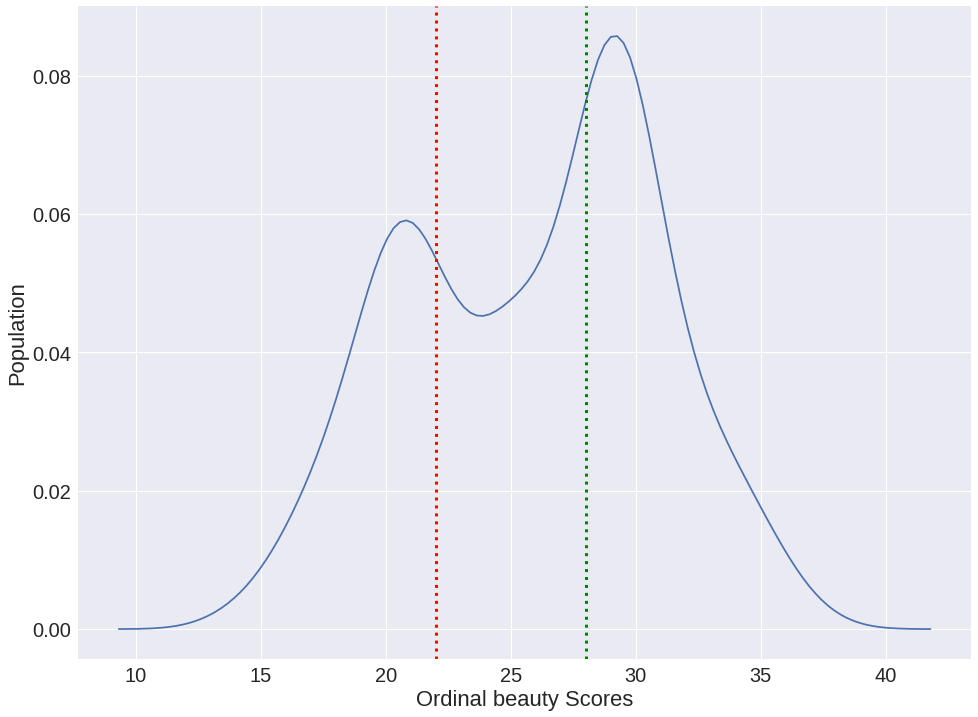
\includegraphics[width=0.7\columnwidth]{Plot/Trueskill.png}
	\caption{Frequency distribution of beauty scores. The red and green lines represent the thresholds below and above which images are considered ugly and beautiful. Conservatively, images in between are discarded.}
	\label{fig:Trueskill}
\end{figure}


\begin{figure*}[t!]
	\centering
	\hspace*{-5mm}
	\subfloat[]{
		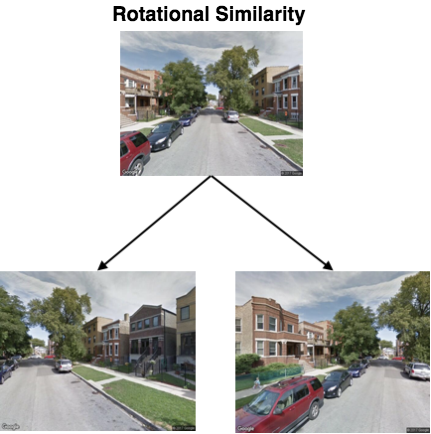
\includegraphics[width=0.5\textwidth, height = 8cm ]{Plot/rotationalSim.png}
		\label{fig:rotSim}
	}
	\subfloat[]{
		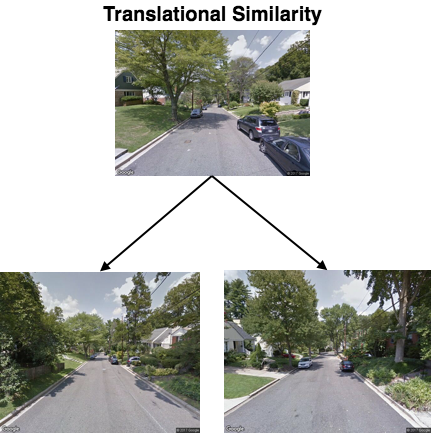
\includegraphics[width=0.5\linewidth, height = 8cm ]{Plot/transSim.png}
		\label{fig:transSim}
	}
	\vspace{-0.4cm}
	\caption{Two types of augmentation: (a) rotation of the Street Views camera (based on rotation); and (b) exploration of scenes at increasing distances (based on translation).}
	\vspace{-0.4cm}
\end{figure*}



\begin{figure}[t!]
	\centering
	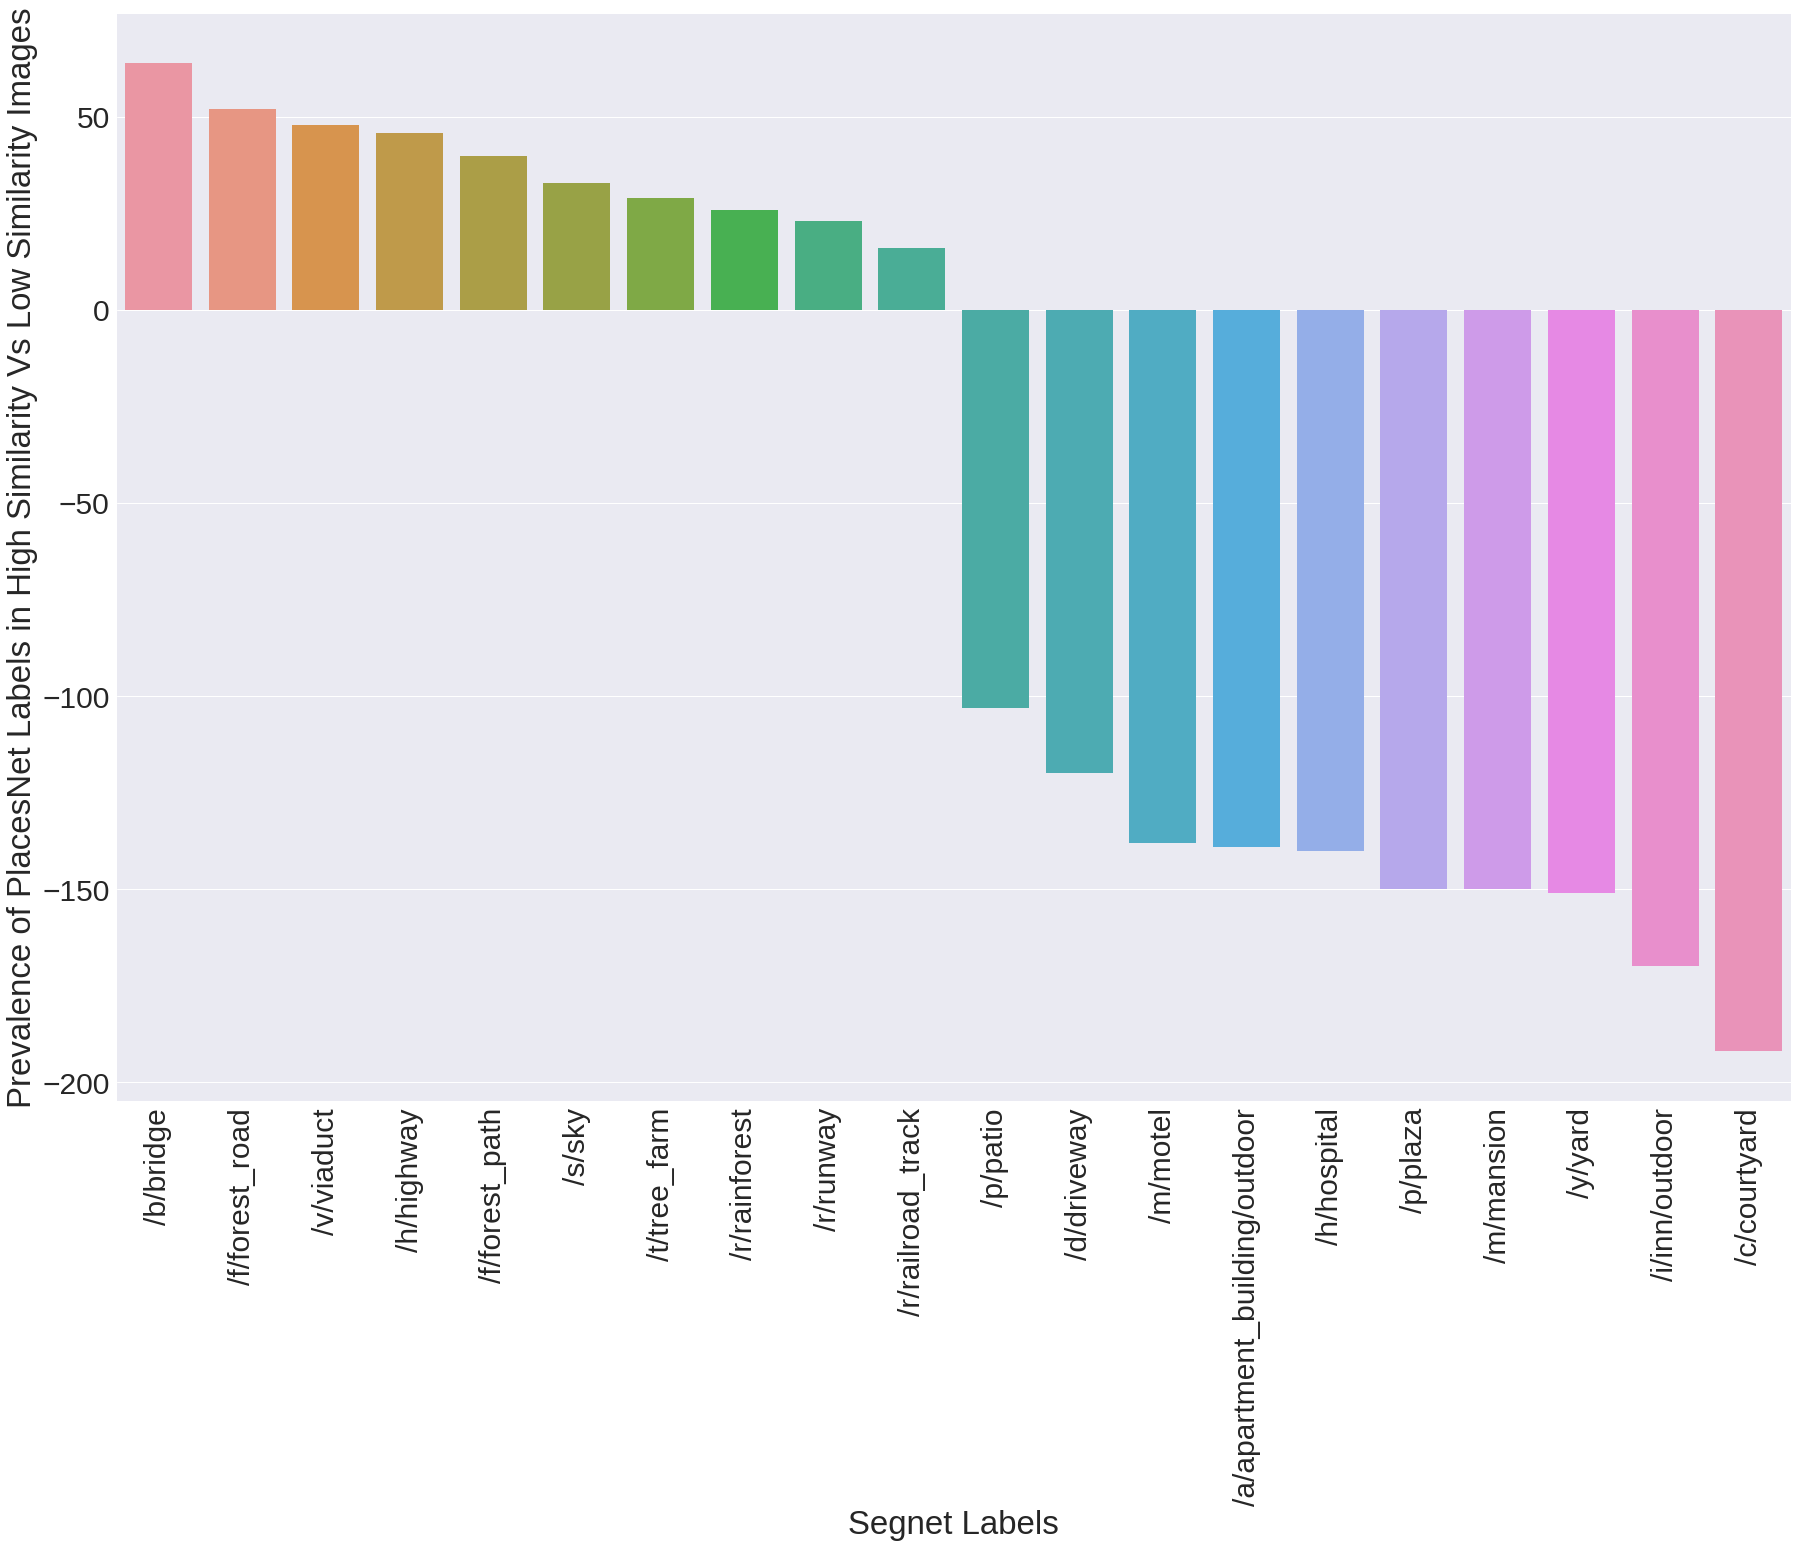
\includegraphics[width=\columnwidth]{Plot/SimilarityPlacesPrevalence.png}
	\caption{The types of scene that have greater propensity to be correctly augmented with similar scenes at increasing distances.}
	\label{fig:augmentationSimilarity}
\end{figure}




\begin{table}[t!]
	\centering
	\begin{tabular}{|c|c|}
		\hline
		\textbf{Augmentation} & \textbf{Accuracy (Percentage)}\\
		\hline
		None & 63 \\
		\hline
		Rotation  & 68 \\
		\hline
		Rotation + Translation  & 64 \\
		\hline
		Rotation + Conservative Translation & 73.5 \\
		\hline
	\end{tabular}
	\caption{Percentage accuracy for our beauty classifier trained on differently augmented sets of  urban scenes.}
	\label{tab:classifier}
    \vspace{-10mm}
\end{table}


%****************************************
\subsection*{Step 2 Training a beauty classifier}
\label{Sec:Classifier}
Having this highly curated set of labeled urban scenes, we are now ready to train classifier $C$ with labels reflecting our beauty assessments. 

As for classifier $C$, we use the CaffeNet architecture, a modified version of AlexNet~\cite{krizhevsky2012imagenet,szegedy2015going}. This has a conventional architecture with 5 convolutional layers; interleaved with  max pooling and normalization layers; and terminated by: \emph{(i)} two 4096 dimensional fully connected layers interleaved with dropout layers~\cite{srivastava2014dropout} (the dropout ratio is set to 0.5 to prevent over-fitting), and \emph{(ii)} by a Softmax layer that classifies the input image into one of two classes of beautiful(1) and ugly(0).  

Having $C$ at hand, we now turn to training it. The training is done on a 70\% split of the data, and the testing on the remaining 30\%. All this is done on increasingly augmented sets of data. We start from our 20k images and progressively augment them with  the snapshots obtained with the 5-angle camera rotations, and then with the exploration of scenes at increasing distance $d \in \{10,20,40,60\}$ meters. The idea behind this data augmentation is that the model's accuracy should increase with increasing levels of augmentation. Indeed it does (Table~\ref{tab:classifier}): it goes from 63\% on the set of original scenes to a value as high as  73.5\% on the set of fully augmented scenes, which is a notable increase in accuracy for this type of classification tasks. Furthermore, our results match previous ones: for example,  Dubey et.al's~\cite{dubey2016deep}  model showed an accuracy of 70\%, which is comparable to ours. 

%As a baseline, we compared with the scenic-or-not model developed by Chanuki et.al \cite{seresinhe2017using}. Their model is different than ours because of the fact that their model generates scenic scores on a scale of 10, whereas ours is a binary classifier. Still for the sake of comparison, we measure the Kendall rank correlation, which is what they use for their measurements, between predicted and actual classes. Our model performs with a Kendall rank correlation of 0.43 which is comparable to their elastic net models. In so far, the facelift pipeline is agnostic of the classifier , which can be swapped out with a better performing one or with one trained for a different use case. 
%\ns{Can you cite a baseline comparison from state of the art? Less important but comment on why is accuracy the right metric? Why not precision for instance?}. 


%\begin{figure*}[h]
%	\centering
%	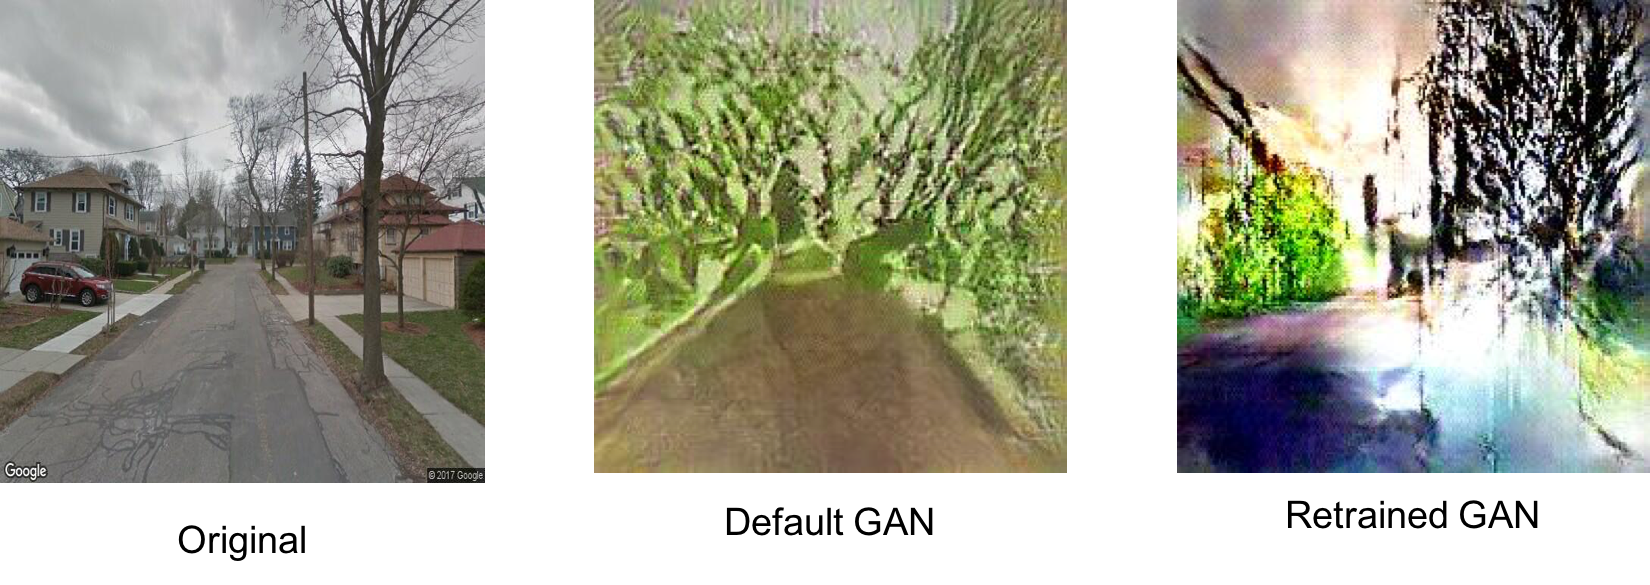
\includegraphics[width=0.5\linewidth]{Plot/GanCompare.png}
%	\caption{Comparison of using the Default ImageNet GAN against Custom trained GAN for Activation maximization. By re-training the GAN on the test dataset, we can see improvement in terms of structure and colours in the generated images}
%	\label{fig:GanComparison}
%\end{figure*}


%****************************************


\subsection*{Step 3 Generating a synthetic beautified scene}

\begin{figure}[t!]
    \centering
    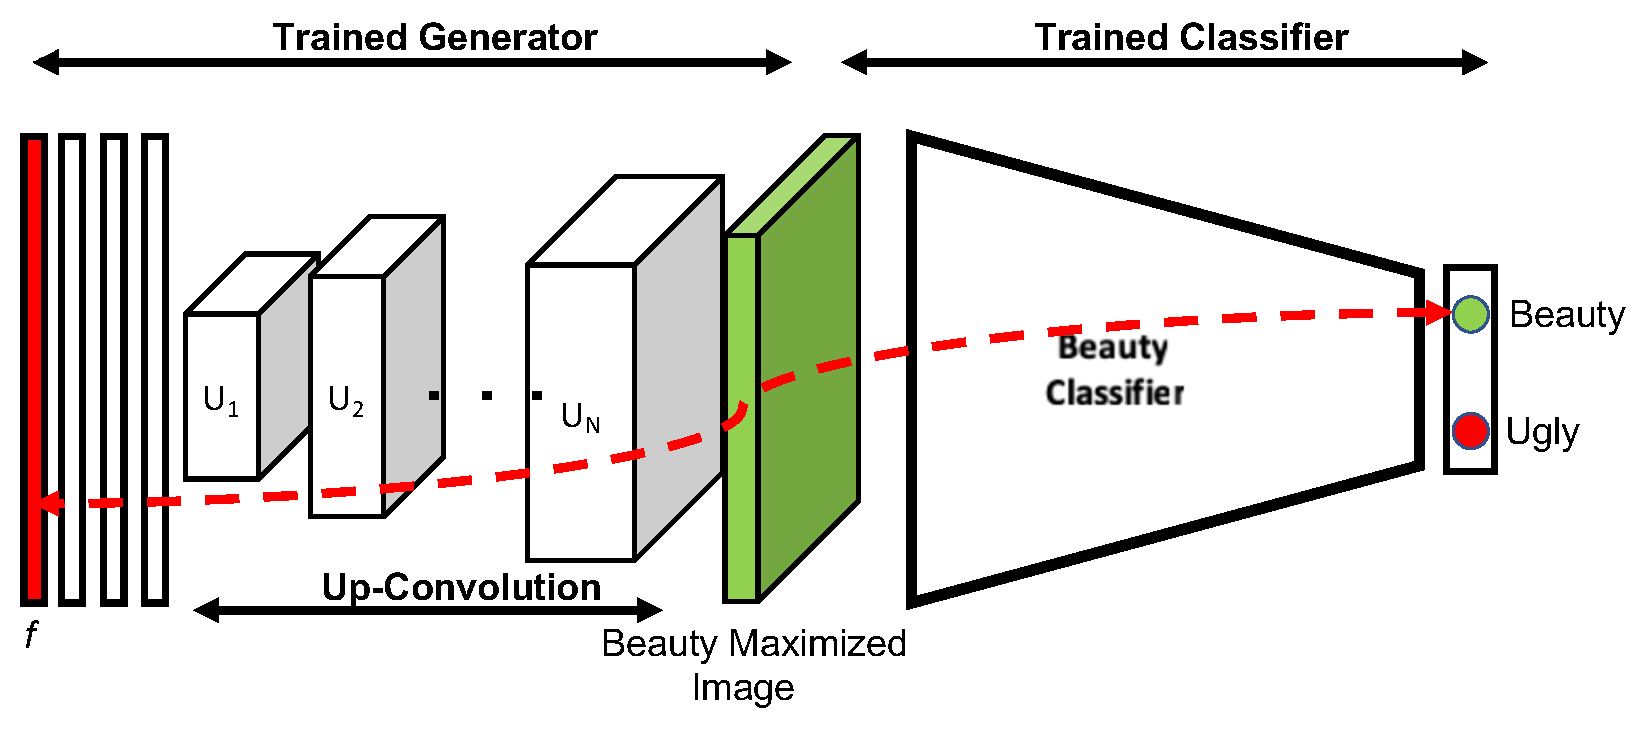
\includegraphics[width=\columnwidth]{Plot/AM_arch.pdf}
    \caption{Architecture of the synthetic beauty generator. This consists of a generator of synthetic scenes concatenated with a beauty classifier. The green block is the beauty maximized template $\hat{I_j}$, which is subject to  forward and backward passes (red arrow) when optimizing for beauty.}
    \label{fig:AM_arch}
\end{figure}

\begin{table}\sffamily
    \begin{tabular}{l*2{C}@{}}
        \toprule
        & Original & Generated \\ 
        \midrule
        & 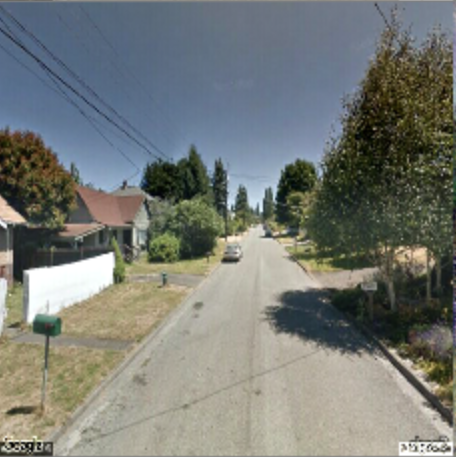
\includegraphics[width=11em]{Plot/GAN_examples/orig_1} & 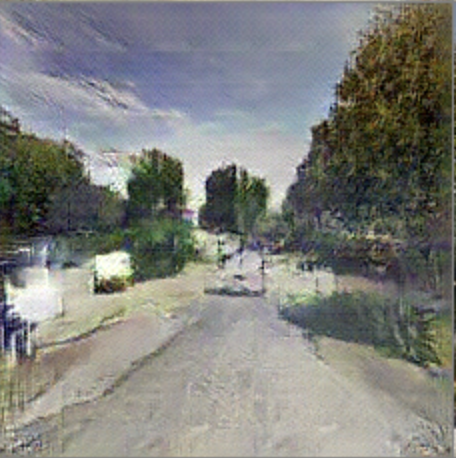
\includegraphics[width=11em]{Plot/GAN_examples/gan_1} \\ 
        & 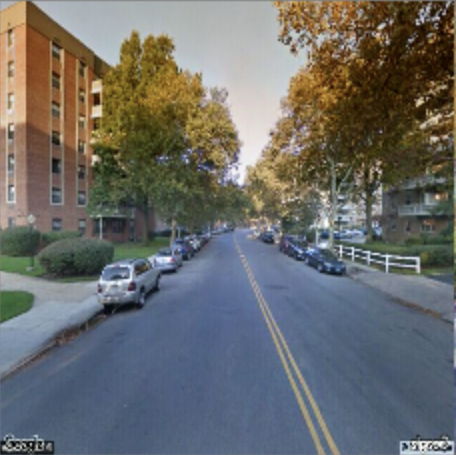
\includegraphics[width=11em]{Plot/GAN_examples/orig_2} & 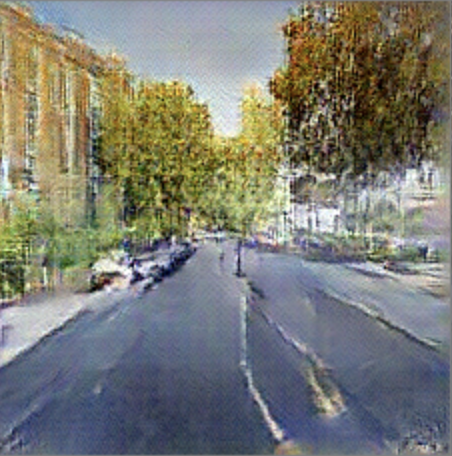
\includegraphics[width=11em]{Plot/GAN_examples/gan_2} \\ 
        & 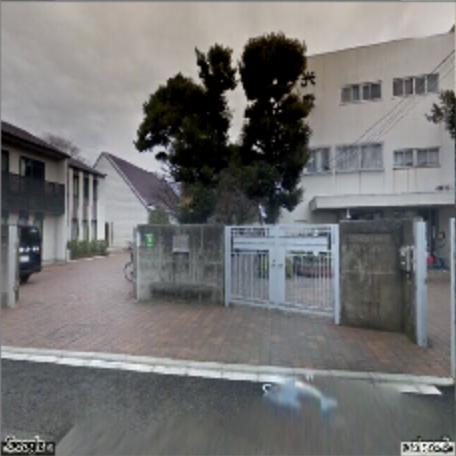
\includegraphics[width=11em]{Plot/GAN_examples/orig_3} & 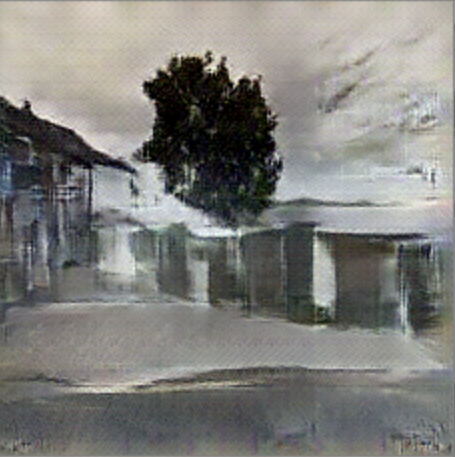
\includegraphics[width=11em]{Plot/GAN_examples/gan_3} \\ 
        
        \bottomrule 
    \end{tabular}
    \caption{Examples of our generator's outputs. The original scenes and the generated ones are shown side by side.}
    \label{fig:GanExample}
\end{table} 


Having this trained classifier at hand, we can then build a generator of synthetic beautified scenes. To build such a generator, we  retrain the GAN described by Dosovitskiy and Brox~\cite{dosovitskiy2016generating} on our curated urban scene dataset. This network is trained by maximizing the confusion for the discriminator between the generated images $G(f)$ and the original ones $I_f$~\cite{goodfellow2014generative}.  The resulting generator is concatenated with our beauty classifier (Figure~\ref{fig:AM_arch}). As a result, given the two classes ugly $y_i$ and beautiful $y_j$, the end-to-end model  transforms any original scene $I_i$ of class $y_i$ (e.g., ugly scene) into template scene $\hat{I_j}$ that maximizes class $y_j$ (e.g., beautified template scene). 

 % able to reproduce synthetic urban scenes (Figure~\ref{fig:GanExample}) 
%to an impressive level of detail. shows a few examples of how the generator performs by comparing a real world image $I_f$, and the generated image $G(f)$. 
%
%
%The second component is a concatenation of  the trained generator with the beauty classifier described in Section~\ref{Sec:Classifier}, as shown in . This results in 

More specifically, given an input image $I_i$ known to be of class $y_i$  (e.g., ugly), our technique outputs  $\hat{I_j}$, which is a more beautiful version of it (e.g., $I_i$ is morphed  towards the average representation of a beautiful scene) while preserving $I_i$'s details. The technique does so using the ``Deep Generator Network for Activation Maximization'' (\emph{DGN-AM})~\cite{nguyen2016synthesizing}. Given an input image $I_i$, \emph{DGN-AM} iteratively re-calculates the color of $I_i$'s pixels in  a way  the output image $\hat{I_j}$  both maximizes  the  activation of neuron $y_j$ (e.g., the ``beauty neuron'') and looks ``photo realistic'',  which is done by conditioning the maximization to an ``image prior''. This is equivalent to finding the feature vector $f$ that maximizes the following expression:
\begin{equation}
\hat{I_j} =G( f ) : \underset{f}{\arg\max}(C_{j}(G(f))-\lambda||f||)
\end{equation}
where:
\begin{itemize}
\item $G(f)$ is the image synthetically generated from the candidate feature vector $f$;
\item $C_j(G(f))$ is the activation value of neuron $y_j$ in the scene classifier $C$ (the value to be maximized);
\item $\lambda$ is a $L_2$ regularization term.
\end{itemize}
Here the initialization of $f$ is key. If $f$ were to be initialized with random noise, the resulting $G(f)$ would be the average representation of category $y_j$ (of, e.g., beauty). Instead, since $f$ is initialized with the feature vector corresponding to $I_i$, then the resulting maximized $G(f)$ is $I_i$'s version ``morphed to become more beautiful''.

The input image is also key. It makes little sense to beautify an already beautiful image, not least because such beautification process would result in a saturated template $\hat{I_j}$ in our framework. For this reason, to generate an image that maximizes the beauty neuron in the classifier $C$, we restrict the  corresponding input image to be in class $y_i$ (i.e., ugly scenes as per the divisions in Figure~\ref{fig:Trueskill}). We do the opposite when maximizing the ugly neuron. 



%Maximizing beauty of an already beautiful urban scene, would yield in a saturated template $\hat{I_j}$. 

%****************************************
\subsection*{Step 4 Returning a realistic beautified scene}
 We now have template scene $\hat{I_j}$ (which is a synthetic beautified version of original scene $I_i$) and need to retrieve a realistic looking version of it. We do so by: \emph{i)} representing each of our original scenes in Step 1 (including $\hat{I_j}$) as a 4096 dimensional feature vector derived from the FC7 layer of the PlacesNet~\cite{zhou2014learning}; \emph{ii)} computing the distance (as $L_2$ Norm) between $\hat{I_j}$'s feature vector and each of the original scene's feature vector; and \emph{iii)} selecting the original scene most similar (smaller distance) to $\hat{I_j}$. This results into the selection of the beautified scene $I_j$.
 
 
 %****************************************
\subsection*{Step 5 Identifying  characterizing urban elements}
Since original scene $I_i$ and beautified scene $I_j$ are real scenes with the  same structural characteristics (e.g., point of view, layout), we can easily compare them in terms of presence or absence of urban elements extracted by computer vision tools such as SegNet and PlacesNet. That is, we can determine how the original scene and its beautified version differ in terms of urban design elements. 
 
 
%\begin{figure*}[h]
%	\centering
%	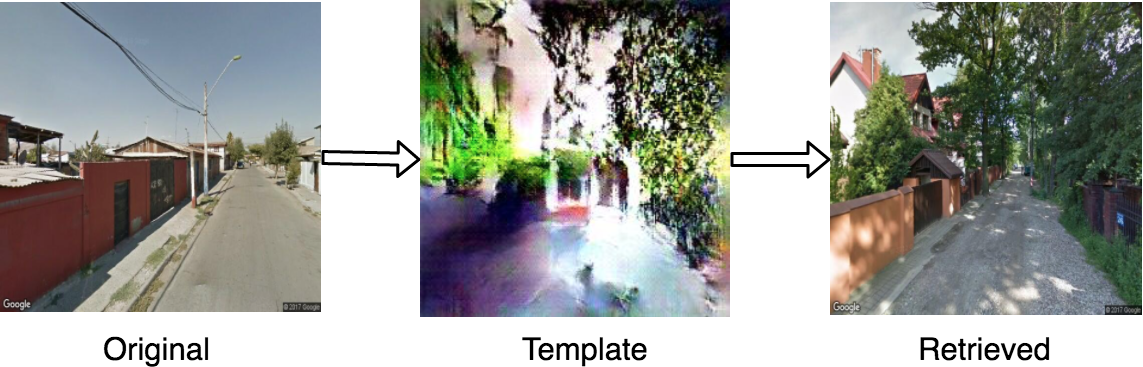
\includegraphics[width=\linewidth]{Plot/Example.png}
%	\caption{Example of ``FaceLifting''.}
%	\label{fig:BeautyExample}
%\end{figure*}


	\begin{table}\sffamily
	\begin{tabular}{l*3{C}@{}}
		\toprule
		 & Original ($I_i$) & Latent Beauty representation ($\hat{I_j}$) & Beautified ($I_j$) \\ 
		\midrule
		& 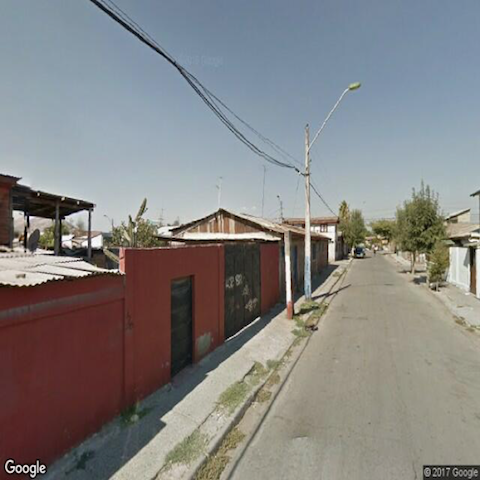
\includegraphics[width=11em]{Plot/examples/u_9} & 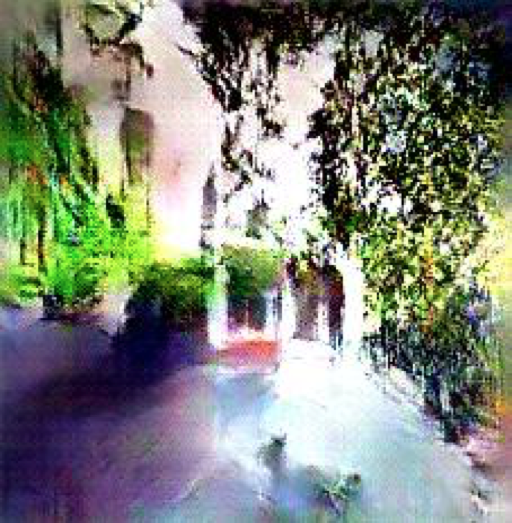
\includegraphics[width=11em]{Plot/examples/t_9} &  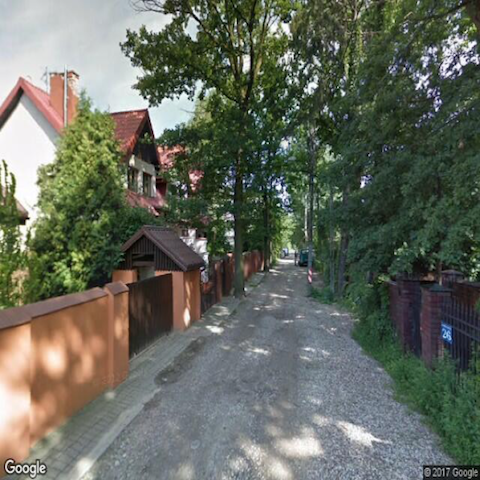
\includegraphics[width=11em]{Plot/examples/b_9} \\ 
%		& 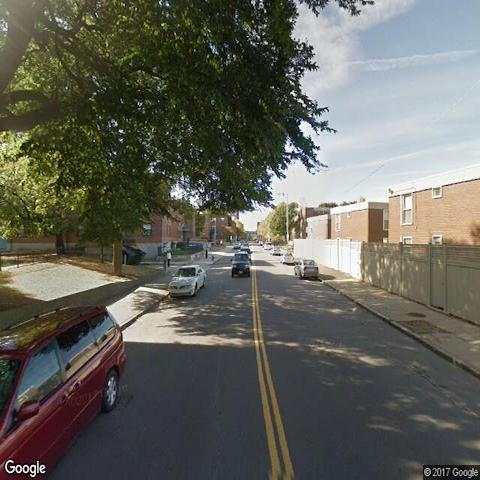
\includegraphics[width=11em]{Plot/examples/u_1} & 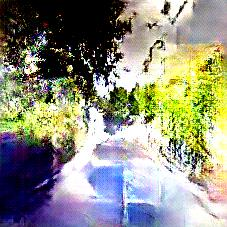
\includegraphics[width=11em]{Plot/examples/t_1} &  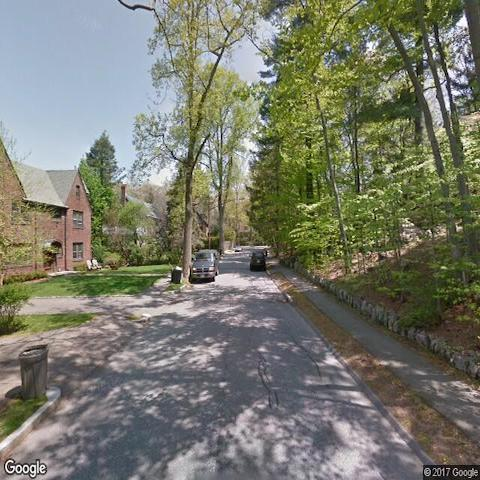
\includegraphics[width=11em]{Plot/examples/b_1} \\ 
%		& 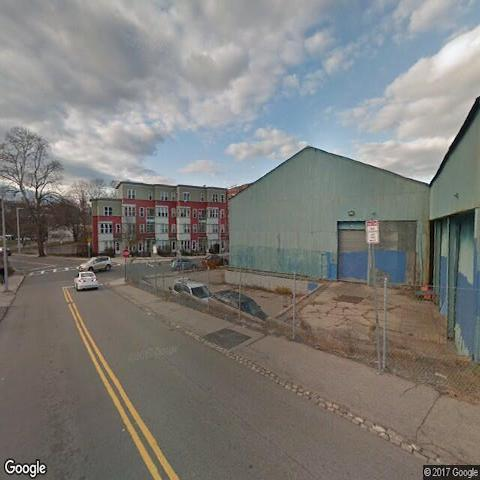
\includegraphics[width=11em]{Plot/examples/u_2} & 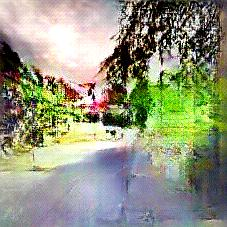
\includegraphics[width=11em]{Plot/examples/t_2} &  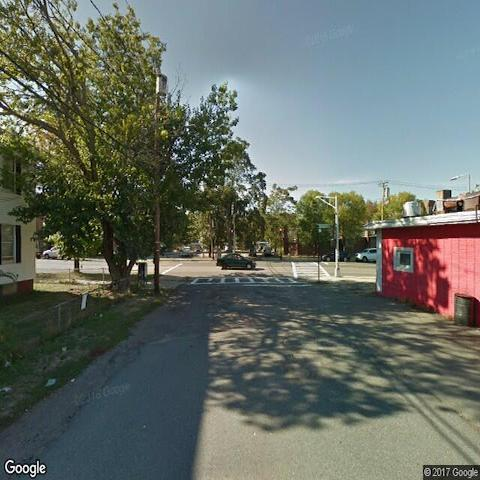
\includegraphics[width=11em]{Plot/examples/b_2} \\ 
%		& 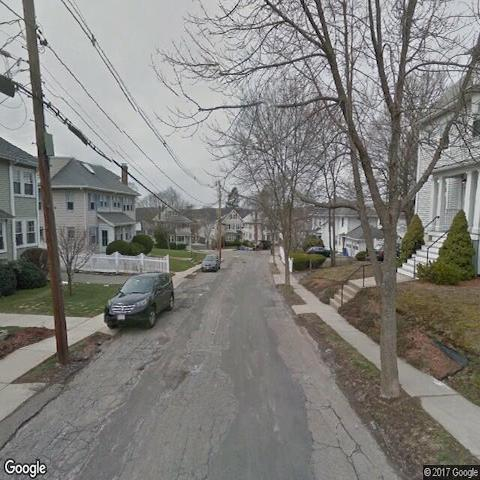
\includegraphics[width=11em]{Plot/examples/u_3} & 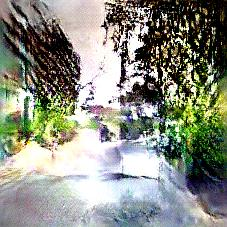
\includegraphics[width=11em]{Plot/examples/t_3} &  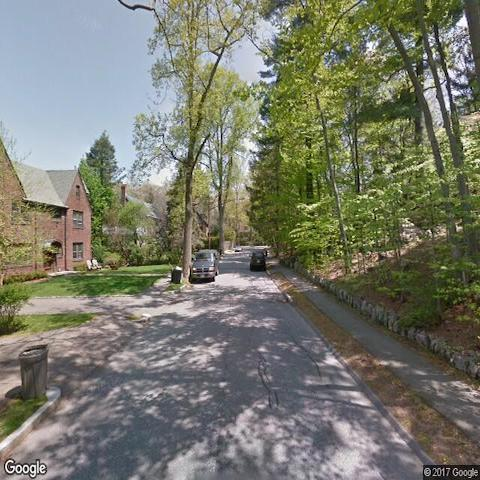
\includegraphics[width=11em]{Plot/examples/b_3} \\ 
		& 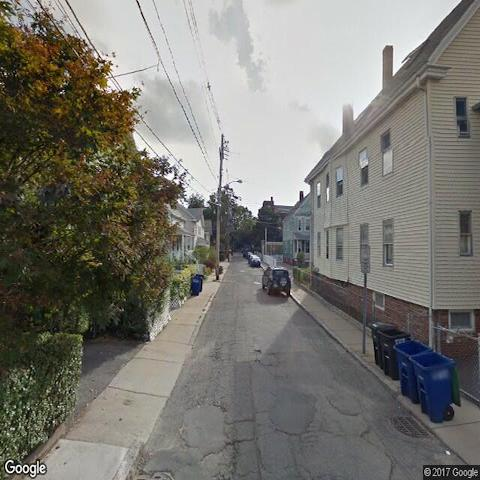
\includegraphics[width=11em]{Plot/examples/u_4} & 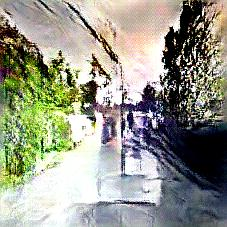
\includegraphics[width=11em]{Plot/examples/t_4} &  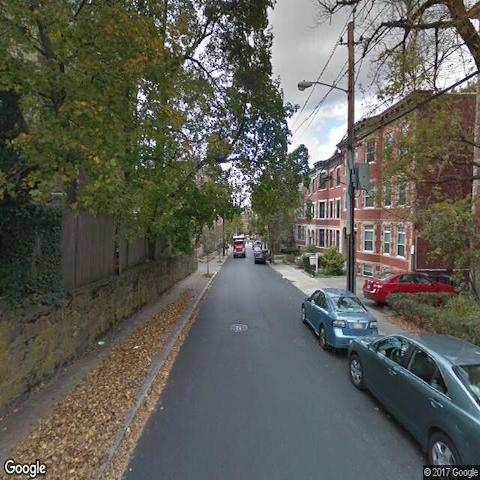
\includegraphics[width=11em]{Plot/examples/b_4} \\ 
		& 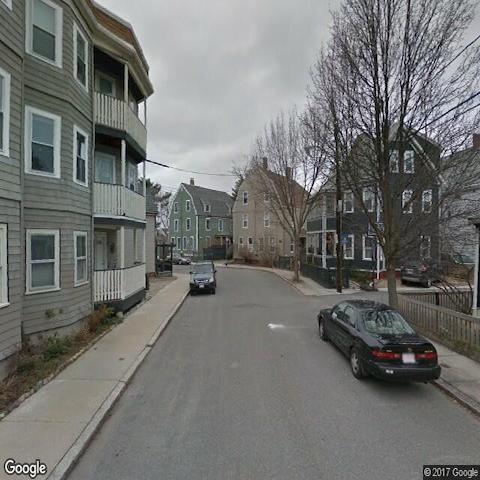
\includegraphics[width=11em]{Plot/examples/u_5} & 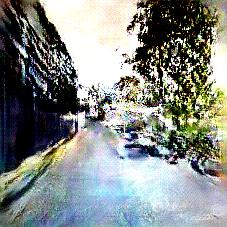
\includegraphics[width=11em]{Plot/examples/t_5} &  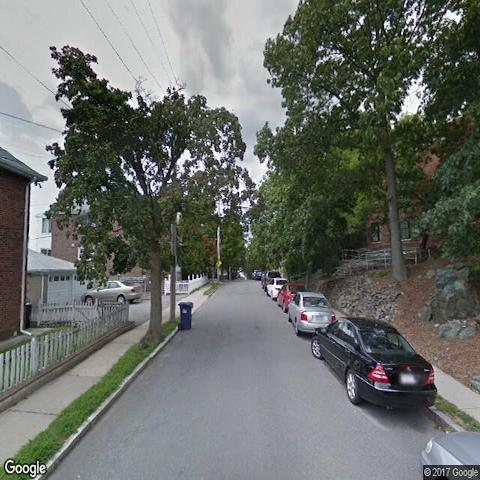
\includegraphics[width=11em]{Plot/examples/b_5} \\ 
%		& 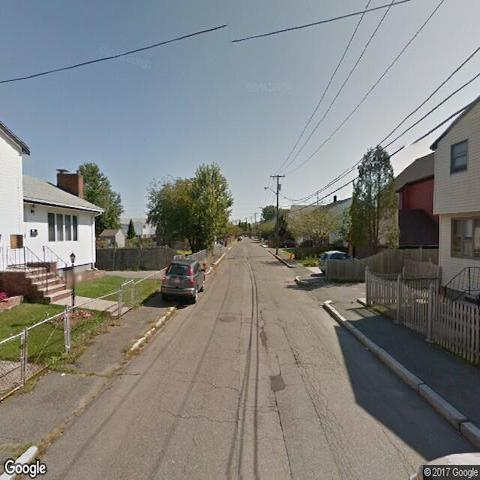
\includegraphics[width=11em]{Plot/examples/u_6} & 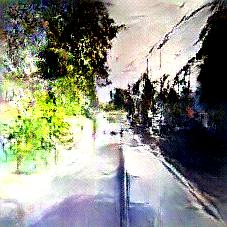
\includegraphics[width=11em]{Plot/examples/t_6} &  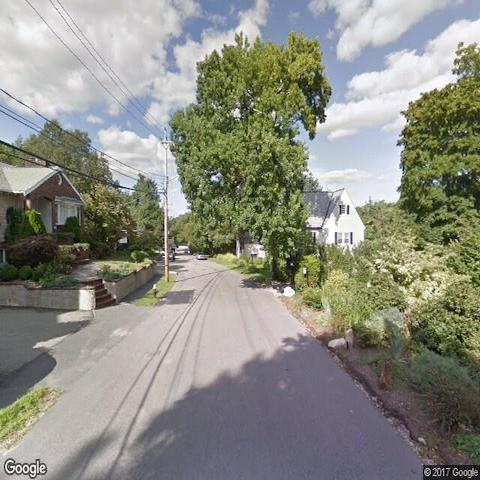
\includegraphics[width=11em]{Plot/examples/b_6} \\ 
		& 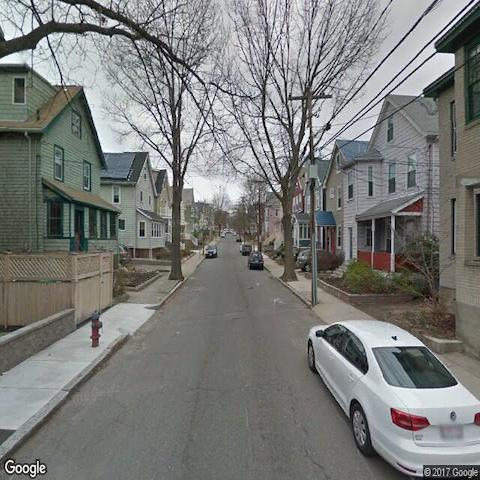
\includegraphics[width=11em]{Plot/examples/u_7} & 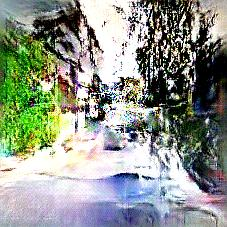
\includegraphics[width=11em]{Plot/examples/t_7} &  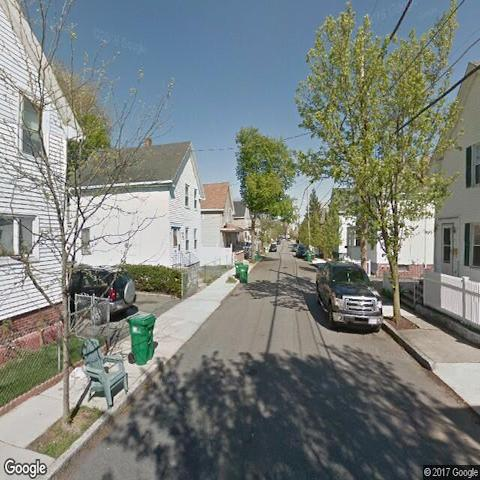
\includegraphics[width=11em]{Plot/examples/b_7} \\ 
		& 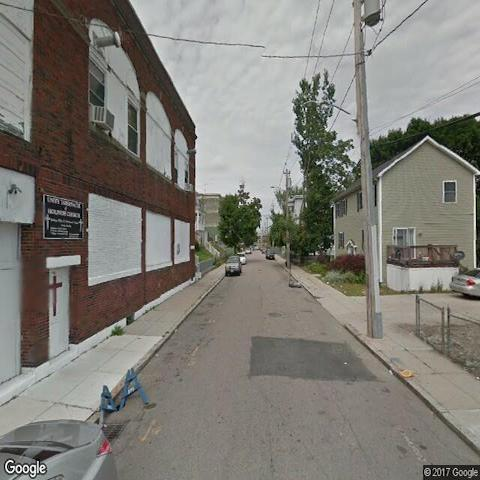
\includegraphics[width=11em]{Plot/examples/u_8} & 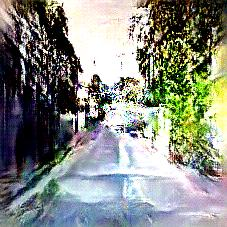
\includegraphics[width=11em]{Plot/examples/t_8} &  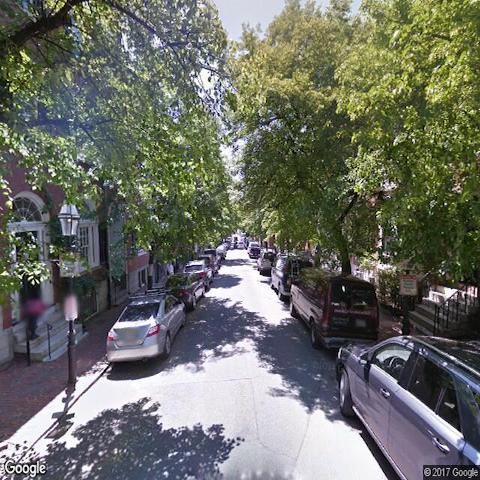
\includegraphics[width=11em]{Plot/examples/b_8} \\ 
		\bottomrule 
	\end{tabular}
	\caption{Examples of the ``FaceLifting'' process, which tends to add greenery, narrow roads, and  pavements.}
	\label{fig:BeautyExample}
\end{table} 

